\documentclass[a4paper, 11pt]{article}
\usepackage{enumitem}
\usepackage{geometry}
\usepackage{amsmath}
\geometry{letterpaper, margin=1in}
\usepackage{graphicx}
\graphicspath{ {images/} }
\usepackage{pdfpages} % for including full pdf pages




% change margins for solution
\newenvironment{solution}{%
	\begin{list}{}{%
			\setlength{\topsep}{0pt}%
			\setlength{\leftmargin}{0.5cm}%
			\setlength{\rightmargin}{0.5cm}%
			\setlength{\listparindent}{\parindent}%
			\setlength{\itemindent}{\parindent}%
			\setlength{\parsep}{\parskip}%
		}%
		\item[]}{\end{list}}


\begin{document}




\begin{enumerate}[leftmargin=0em, label=\textbf{\arabic*}.]
  \item The potential due to a ring of charge is given by:
    \[
      V(s,\phi,z) = \frac{1}{4\pi\epsilon_0}\frac{Q}{2\pi}\int_0^{2\pi}\frac{d\phi'}{\sqrt{s^2+R^2-2sR\cos(\phi-\phi')+z^2}}
    \]
    Expand this potential in a power series to fourth order, in the plane of the
    ring, for $s<R$. Warning: Make sure you keep \textbf{all} of the terms up to
    fourth order and none of the terms of higher order. This is tricky to do and
    is the most important lesson from this homework problem. \\
\end{enumerate}

\noindent\textbf{Solution:}
\begin{solution}
  \noindent To expand this potential in a power series, it would be nice to save
  some effort and use the series we have already memorized (Quiz 1). Recall,
  \begin{equation}
    (1+u)^p = 1+pu + \frac{p(p-1)}{2!}u^2+\frac{p(p-1)(p-2)}{3!}u^3+\frac{p(p-1)(p-2)(p-3)}{4!}u^4+ \cdots
  \end{equation}
  We are looking at the potential in the plane of the ring, so $z=0$. We can
  also rewrite the square root as a power.
  \begin{equation}
    V(s,\phi,z=0)=\frac{1}{4\pi\epsilon_0}\frac{Q}{2\pi}\int_0^{2\pi}\Big(s^2+R^2-2sR\cos(\phi-\phi')\Big)^{-1/2}d\phi'
  \end{equation}
  The integrand is almost the same as equation (1) but we need it to match
  exactly for the power series to be valid. \textbf{Remember:} equation (1) is
  valid only for $|u|<1$. We are interested in finding the potential where
  $s<R$, or in other words, $s/R<1$ is a small quantity and we can \textit{pull
    out} $R^2$ from the expression. That is,
  
  \begin{align}
    \Big(s^2+R^2-2sR\cos(\phi-\phi')\Big)^{-1/2} &= \Big[R^2\Big(1+\frac{s^2}{R^2}-\frac{2s}{R}\cos(\phi-\phi')\Big)\Big]^{-1/2}\\
                                                 &= \frac{1}{R}\Big(1+\frac{s^2}{R^2}-\frac{2s}{R}\cos(\phi-\phi')\Big)^{-1/2} 
  \end{align}
  \begin{equation}
    u \equiv \frac{s^2}{R^2}-\frac{2s}{R}\cos(\phi-\phi'), \qquad p=-1/2
  \end{equation}
  where in the final line I have identified our $u$ and $p$ for the series
  expansion. \\
  
  \noindent Now, we need to expand the powers of $u$ in order to find all of the fourth
  order terms in $\frac{s}{R}$. Yes, this is a lot of algebra. 
  \begin{align}
    &p(u) =  \left( \frac{s}{R} \right)\cos(\phi-\phi')-\frac{1}{2}\left( \frac{s}{R} \right)^2\\
    &\frac{p(p-1)}{2!}u^2 = \frac{5}{2}\left( \frac{s}{R} \right)^2\cos^2(\phi-\phi')-\frac{3}{2}\left( \frac{s}{R} \right)^3\cos(\phi-\phi')+\frac{3}{8}\left( \frac{s}{R} \right)^4 \\
    & \frac{p(p-1)(p-2)}{3!}u^3 = \frac{5}{2}\left( \frac{s}{R} \right)^3\cos^3(\phi-\phi')-\frac{15}{4}\left( \frac{s}{R} \right)^4\cos^2(\phi-\phi/) +...\\
    & \frac{p(p-1)(p-2)(p-3)}{4!}u^4 = \frac{35}{8}\left( \frac{s}{R} \right)^4\cos^4(\phi-\phi')+...
  \end{align}
  Using this to combine all terms with like powers in $s/R$, the integral reduces to
  \begin{equation}
    \begin{split}
      V(s,\phi)\approx\frac{1}{4\pi\epsilon_0}\frac{Q}{2\pi}\frac{1}{R}\int_0^{2\pi}&\Bigg\{ 1+\cos(\phi-\phi')\left( \frac{s}{R} \right)\\
      &+ \left[ \frac{3}{2}\cos^2(\phi-\phi')-\frac{1}{2}  \right]\left( \frac{s}{R} \right)^2\\
      &+ \left[ \frac{5}{2}\cos^3(\phi-\phi')-\frac{3}{2}\cos(\phi-\phi')    \right]\left( \frac{s}{R} \right)^3\\
      &+ \left[ \frac{3}{8}-\frac{15}{4}\cos^2(\phi-\phi')+\frac{35}{8}\cos^4(\phi-\phi') \right]\left( \frac{s}{R} \right)^4  \Bigg\}d\phi'
    \end{split}
  \end{equation}

  \noindent The original equation for the potential can not be integrated analytically.
  Now that we have expanded the integrand, we have reduced the problem to a
  bunch of integrals of $\cos^n(\phi-\phi')$ which we can solve by 
  brute force. If you wish to do the integrals by hand, take advantage of the
  exponential form of cosine. Otherwise, Mathematica is a great option for this
  sort of integral. \\


  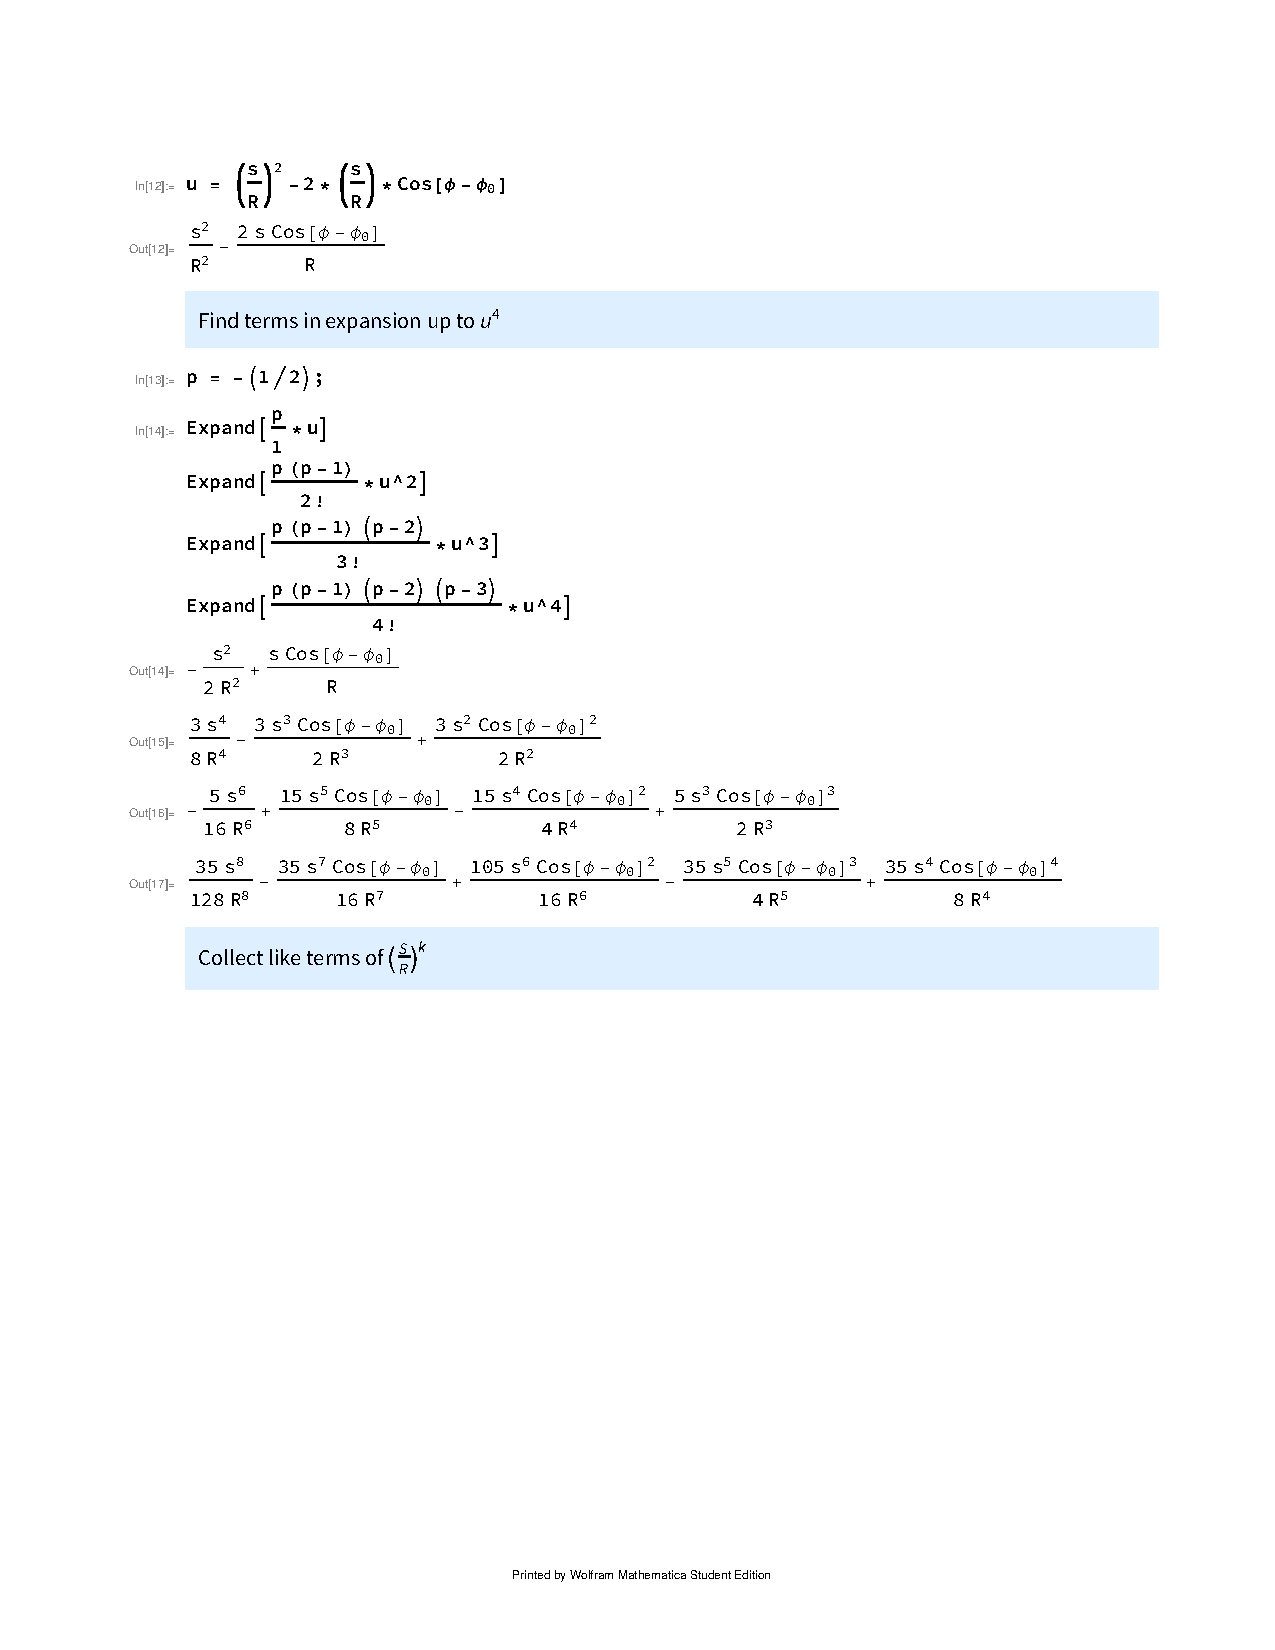
\includepdf[pages=-]{mathematica_integral.pdf}

  
  % \begin{figure}[!hbt]
  %   \centering
  %   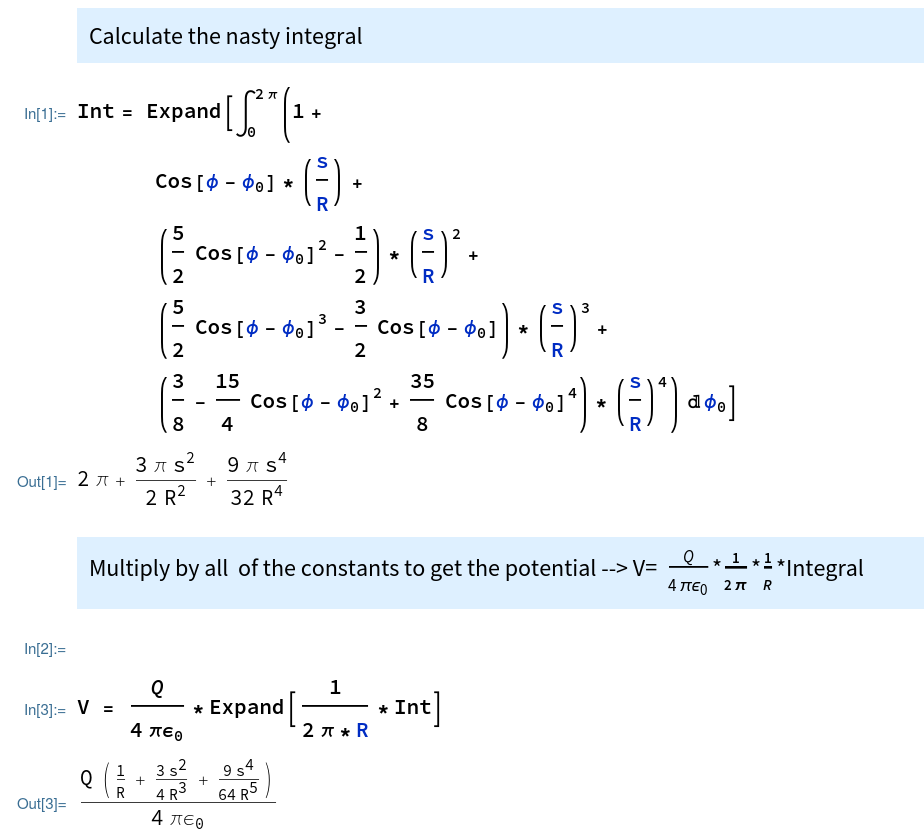
\includegraphics[width=1.0\columnwidth]{mathematica_integral}
  % \end{figure}

  
  \noindent Therefore, our solution for the electric potential in the plane of the ring to
  fourth order in $s$ is
  \begin{equation}
    V(s,\phi,z=0) \approx \frac{Q}{4\pi\epsilon_0}\Bigg\{  \frac{1}{R} + \frac{1}{4} \frac{s^2}{R^3}+\frac{9}{64} \frac{s^4}{R^5} \Bigg\} 
  \end{equation}
  

  \vspace{2em}
  
  \noindent\textbf{NOTE:} Our solution does not depend on $\phi$ \textit{and}  is an even function in $s$. Why is that? \\

  \noindent\textbf{CHECK:} Does our solution agree with the original integral equation at
  the origin? 
  
\end{solution}

\end{document}





















